\documentclass[11pt]{article}
\usepackage{graphics}
\usepackage{graphicx} %So we can include .png and .jpg files
\usepackage{url}
\usepackage{verbatim}
\usepackage{fullpage} %Cause it sucks when math runs off the page
\usepackage{makeidx}
\usepackage{html}

\makeindex
%I don't like my paragraphs indented because we have lots of 1-line paragraphs with URLs or code after them
\setlength{\parindent}{0in} 
%I like space between my paragraphs
\setlength{\parskip}{10pt} 


\title{RL-Glue 3.0 Overview}
\author{Adam White :: awhite@cs.ualberta.ca}
\date{}

\begin{document}
\maketitle
\tableofcontents


\section{Introduction}
\subsection{Purpose of Document}
This document has been laid out so that it can be used for: 
\begin{enumerate}
\item  {\bf RL-Glue what?} learning about RL-Glue at an abstract level
\item {\bf Compatibility:} help convert existing and environments work with RL-Glue
\item {\bf Plugging agents and environments together:} how to write experiment programs
\item{\bf What function do I use to:} quick function reference for RL-Glue
\end{enumerate}

In September 2008, the RL-Glue Project was split into two projects: RL-Glue and RL-Glue Extensions.

RL-Glue now only includes the RL-Glue interface and plugs for direct-compile C/C++ agents, environments and experiment programs.

The RL-Glue Extensions Project contains codecs that allow C/C++, Java, Python, Matlab, and Lisp agents/environments/experiments to use RL-Glue.  This multi-language support was previously bundled with RL-Glue.  The reason for the split was partially to separate the technical details of using RL-Glue with a particular language from the high level overview of what RL-Glue does.

This document is the high-level overview document: it contains contains {\bf NO} implementation specific technical details for writing programs.

Please refer to the \htmladdnormallink{RL-Glue technical manual}{http://rl-glue.googlecode.com/svn/trunk/docs/tech_html/index.html} and \htmladdnormallink{manuals for specific codecs}{http://glue.rl-community.org/Home/Extensions} for language specific details on how to implement agents, environments and experiment programs.
 
\subsection{How to Use This Document}

This document as been divided to reflect the purposes described above. To learn about the major components of RL-Glue and a description of how those components interact see Section \ref{RL-Glue}. To learn how to make environment and agent programs compatible with RL-Glue we recommend sections \ref{envp1} and \ref{agentp1}. Sections \ref{envp1} and \ref{agentp1} describe only the mandatory functions that RL-Glue environments and agents must implement. Sections \ref{envp2} and \ref{agentp2} describe advanced environment and agent functions. To learn about experiment programs and how they interact with RL-Glue see Section \ref{exp}. For quick function reference see Section \ref{ref}. Frequently asked questions can be found in Section \ref{faq}. A summary of and explanations for all changes from RL-Glue 2.X to RL-Glue 3.0 can be found in Section \ref{change}.

RL-Glue uses naming conventions and definitions from Sutton and Barto's text: ``Reinforcement Learning: An Introduction".  This text is available for free online: \url{http://www.cs.ualberta.ca/~sutton/book/the-book.html}.
 
 
\section{RL-Glue Concepts}
\label{RL-Glue}
A large part of studying and researching reinforcement learning is experimentation. When you write an agent, you should ensure the agent makes exploratory moves to discover more about the world. Similarly, it is important that you are able to ``explore'' new algorithms and ideas without having to create the experiment code for each test. One of the goals of RL-Glue is to simplify and accelerate the process of writing an experiment so that many ideas can be easily tested. 


In machine learning research, it is important to look at other work being done in the field, compare your own performance and then improve. One goal for RL-Glue is to provide a consistent tool for using and comparing agents and environments from diverse sources. A common problem for researchers arises when they try compare their work with previously published results.

Before RL-Glue, the solution was often to reverse engineer code for the experiment based on the results and (often incomplete) implementation descriptions that had been published.  Even code was released to the public, it was often still a challenge to understand adapt the original code. Now, you can make the necessary RL-Glue agent/environment/experiment programs  available to the public such that another experimenter can reproduce your original experiment and easily experiment with their own code to compare performance.  Several recent reinforcement competitions, at \htmladdnormallink{NIPS}{http://rlai.cs.ualberta.ca/RLAI/rlc.html} and \htmladdnormallink{ICML}{http://rl-competition.org} have used RL-Glue for benchmarking participant submissions, further exemplifying the utility of RL-Glue to the research community.
 
\begin{figure}
	\begin{centering}
%\htmlimage{scale=0.5}
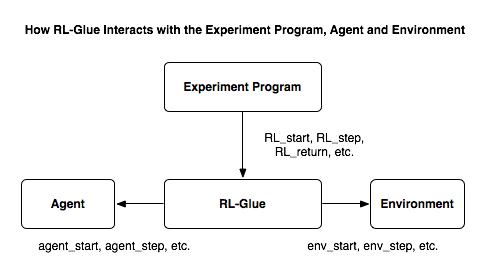
\includegraphics[height=60mm]{images/glue_connections_no_shadow.png}
\caption{The RL-Glue Standard. Arrows indicate function call direction.}
\label{fig:glue-connections}
\end{centering}
\end{figure}

RL-Glue is both a set of ideas and standards, as well as a software implementation. In theory, RL-Glue is a protocol for the reinforcement learning community to follow. Having this very simple standard of necessary functions facilitates the exchange and comparison of agents and environments without limiting their abilities. As software, RL-Glue is functionally a test harness to ``plug in'' agents, environments and experiment programs without having to continually rewrite the connecting code for these pieces. An experiment program is, very simply, code stating how many times to run an agent in an environment and what data should be extracted this interaction. Provided the agent, environment, and experiment program follow the RL-Glue protocol, by implementing the few necessary functions, they can easily be plugged in with the RL-Glue code to have an experiment running quite effortlessly. Figure \ref{fig:glue-connections} is a diagram which shows how function calls work in RL-Glue.



The Experiment Program contains the ``main function'' which will make all of the requests for information through RL-Glue. These requests are usually related to setting up, starting and running the experiment and then gathering data about the agent's performance. The experiment program can never interact with the agent or environment directly: all contact goes through the RL-Glue interface.  There is also no direct contact between the agent and the environment. Any information the agent or environment returns is passed through RL-Glue to the module which needs it.  



\subsection{Agents, Environments and Experiment Programs}
Understanding the semantics we ascribe to \textit{agents}, \textit{environments}, and \textit{experiments} is a fundamental part of understanding RL-Glue.

In RL-Glue, the \textit{agent} is both the learning algorithm and the decision maker. The agent decides which action to take at every step.

The \textit{environment} is responsible for storing all the relevant details of the world, or problem of your experiment. The environment generates the observations/states/perceptions that are provided to the agent, and also determines the transition dynamics and rewards.  

The experiment is the intermediary which (through RL-Glue) controls all communication between the agent and environment.  This structured separation is by design, division of the agent and environment both helps create modularized code and captures our intuitions about how much the agent and environment should ``know'' about each other.

The experiment program will be familiar to anyone who create reinforcement learning experiments. Akin to the typical main function in many reinforcement learning experiments, an RL-Glue experiment program is a control loop which runs the agent through the environment {\bf x} number of times, perhaps doing {\bf y} trials of these {\bf x} episodes, all the while gathering data about how efficiently the agent has behaved or how quickly it has learned. RL-Glue provides several functions (Section \ref{ref}) to assist in writing an experiment program.



\section{RL-Glue Environment Programs}
\label{env}
The environment represents everything outside the agent's direct control. For example, in a tabular grid world, the environment determines the state space, the obstacles, the rewards, start states, termination conditions and the state transitions.  In a robotic task, the environment would also include the robot's body, because the agent does not have complete, deterministic control over its motors. The environment is basically everything that is not the agent.

In RL-Glue, the environment is defined by a set of parameterized functions that the RL-Glue interface queries on behalf of the experiment program. These functions define what the environment does before an experiment begins, at the beginning of an episode, on every remaining step of the episode and after the experiment is completed. The following sections describe the basic requirements of an RL-Glue environment and present a complete list of all environment functions.

\subsection{Essential Components Of A RL-Glue Environment}
\label{envp1}

Every RL-Glue environment must implement a number of functions.  The most important functions are \texttt{env\_start} and \texttt{env\_step}.   

\subsubsection{Observation and Action Encoding}
In RL-Glue, Observations, Actions, and some other types are represented by structures that are any combination of:
\begin{itemize}
\item list of discrete numbers (\texttt{int})
\item list of continuous numbers (\texttt{double})
\item list of ASCII characters
\end{itemize}

We have found that most action an observation types can easily be captured with this structure.  In a grid world, for example, the action can be an \texttt{int} list of length 1 (with valid values 0-3), corresponding to (N,S,E,W) and the observation can also be an \texttt{int} list of length 1 that maps to the agent's current state label (which is also the state of the environment, in this case). In a problem like Mountain Car, the actions are discrete (0-2) and the observation is the car's position and velocity (both real numbers). The action can be an \texttt{int} list of length 1 and the observation can be a \texttt{double} list of length two. Different implementation languages will use different languages constructors to encode observations and actions: please refer to the codec specific manual for your programming language of  choice for more details.

\subsubsection{Environment Start}
The \texttt{env\_start} function is very simple. The function takes no input and simply returns an observation. The \texttt{env\_start} function is the first function called at the beginning of an episode; \texttt{env\_start} chooses the initial state of the environment and returns the corresponding observation. For example, the following pseudocode selects a random start state for a grid world and returns the observation:
\begin{verbatim}
1. env_start -> observation
2.      state = rand()*num_states
3.      set observation equal to state
4. return observation
\end{verbatim}


\subsubsection{Environment Step}
The other essential piece of a RL-Glue environment is the \texttt{env\_step} function. The \texttt{env\_step} function must take an action, as input, and return a observation, a reward and a termination flag. In most reinforcement learning problems, the  \texttt{env\_step} function updates the internal state of the environment, tests for end of episode and returns the new observation of state and current reward. In other words, step function encodes the state transition and reward functions. Keeping with the grid world example, the following would be a valid \texttt{env\_step} function:
\begin{verbatim}
1. env_step(action) -> reward, observation, flag 
2.      newState = updateState(action, state)
3.      flag = isTerminal(newState)
3.      reward = calculate reward for netState
4.      set observation equal to newState
5.      state = newState
6. return reward, observation, flag
\end{verbatim}
Here we assume the existence of a state update function and an isTerminal function that checks if the current state is a terminal state.

So thats it. Just fill in two functions and you have a valid RL-Glue environment. In later sections we will discuss advanced environment functions and how these additional functions can be used to write more complex experiment programs. 

\subsection{Additional Components Of A RL-Glue Environment}
\label{envp2}

So far we have only scratched the surface of what you can do with RL-Glue environments. Additional environment functions can be used to initialize data structures, get and set the state of the environment, get and set the random seed and send generic string messages to the environment. Before we go on describing these functions it is useful to understand the \texttt{task\_spec} language that is used, in RL-Glue, to encode basic information about environments. 

\subsubsection{Task Specification Language (\texttt{task\_spec})}
\label{task}
In an effort to provide the agent writer with simple and concise information about the environment, a \texttt{task\_spec} is passed from the environment, through RL-Glue, to the agent. The environment's init function (\texttt{env\_init}) encodes information about the problem in an ASCII string. The string is then passed to the agent's init function (\texttt{agent\_init}).  This information can also be used to check if an agent and environment pair are compatible. The agent is responsible for parsing any relevant information out of the \texttt{task\_spec} in the \texttt{agent\_init}  function. 

More specifically, the \texttt{task\_spec} string encodes a version number, the number of observation action dimensions, the types of observations and actions, the ranges of the observations and actions and the min and max reward values. 

The \texttt{task\_spec} is constantly evolving to match the state-of-art of learning algorithms and tasks being solved in reinforcement learning research; we expect that the \texttt{task\_spec} will evolve much faster than the main RL-Glue protocol.  To prevent this document from becoming quickly outdated, we have separated the \texttt{task\_spec} documentation from the main RL-Glue documentation. Please see the \htmladdnormallink{online \texttt{task\_spec} documentation}{http://glue.rl-community.org/Home/rl-glue/task-spec-language} for details about different \texttt{task\_spec} versions.

%
%The \texttt{task\_spec} is stored as a string with the following format:
%\begin{verbatim}
%     "V:E:O:A:R"
%\end{verbatim}		
%For example, this is a sample \texttt{task\_spec} provided as one of the examples below:
%\begin{verbatim}
%     "2:e:1_[i]_[0,N-1]:1_[i]_[0,3]:[-1,0]"
%\end{verbatim}     
%The V corresponds to the version number of the \texttt{task\_spec} language. E corresponds to the type of task being solved. It has a character value of `e' if the task is episodic and `c' if the task is continuing. O and A correspond to Observation and Action information respectively. Finally, the R corresponds to the range of rewards for the task. Within each of O, A and R a range can be provided, however if the values are unknown or infinite in magnitude, two special input values have been defined.
%\\\\
%The format of O and A are identical. We will describe the form of O only. O contains three components, separated by underscore characters ("\_") :
%\begin{verbatim}        
%     #dimensions_dimensionTypes_dimensionRanges
%\end{verbatim}
%\#dimensions is an integer value specifying the number of dimensions in the Observation space. dimensionTypes is a list specifying the type of each dimension variable. The dimensionTypes list is composed of \#dimensions components separated by comma characters (``,") within square brackets ([x1,x2,x3,..., xn] where xi  represents the ith value). Each comma-separated value in the list describes the type of values assigned to each Observation variable in the environment. In general, Observation variables can have one of the following 2 types:
%\begin{verbatim}
%     `i' - integer value
%     `f' - float value
%\end{verbatim}
%Thus a dimensionTypes list corresponding to an Observation space with 1 dimension has the following form:
%\begin{verbatim}
%     [a] where a is an element of [`i',`f']
%\end{verbatim}
%So a dimensionTypes list with one integer value would be:    
%\begin{verbatim}    
%     [i]
%\end{verbatim}     
%An Observation space with 2 dimensions would have a dimensionTypes with the following form:
%\begin{verbatim}
%     [a,b] where a and b are elements of [`i',`f']
%\end{verbatim}
%indicating the value type of the first (a) and second (b) Observation variables. Thus a three dimensional Observation with one float, integer dimension and another float dimension would have the following dimensionTypes:
%\begin{verbatim}
%     "[f,i,f]"
%\end{verbatim}
%The dimensionRanges is a list specifying the range of each dimension variable in the Observation space.  The dimensionRanges is composed of \#dimensions components separated by underscore characters. Each dimensionRanges component specifies the upper and lower bound of values for each Observation variable. If the bounds are unknown or unspecified, you can leave an empty space in the place of a value. If the bounds are positive or negative infinity, you can use inf or -inf to represent your range. These can be used in combination. For example one valid range could be an unknown lower bound and infinite upper bound, or a lower bound of -inf and an upper bound of 1. You can be as precise (though you must be accurate) as you wish. A dimensionRanges corresponding to an Observation space with a single dimension variable would have the following form:
%\begin{verbatim}
%     [O1MIN, O1MAX]
%\end{verbatim}
%So a dimensionRanges list for binary dimension varaible would be: [0,1]
%A dimensionRanges list for variable with no upper or lower bound unspecified would be: [] or [,] (both are valid).
%A dimensionRanges with one or two unbounded value can take on a value of inf or -inf. Eg [0, inf] or [-inf,1] or [-inf,inf].
%\\\\
%An Observation space with 2 dimensions would have a dimensionRanges with the following form:
%\begin{verbatim}
%     [O1MIN, O1MAX]_[O2MIN, O2MAX]
%\end{verbatim}
%indicating the minimal and maximal values of Observation variables O1 and O2 respectively. This definition can be then trivially extended to Observation spaces with N dimensions.
%\\\\
%NOTE: the dimensionRanges of an Observation space with 1 or more unbounded values may not be representable in this way. An unbounded value has no minimal or maximal range. Thus, we simply do not specify the range in the dimensionRanges for any Observation variables with unbounded values. For example, consider a problem with 3 Observation dimensions. The first and third Observation variables have interval values and the second has unbounded ratio value. The corresponding dimensionRanges for this problem is encoded as:
%\begin{verbatim}
%     [O1MIN, O1MAX]_[,]_[O3MIN, O3MAX]
%\end{verbatim}
%indicating the minimal and maximal values of Observation variables O1 and O3.
%\\\\
%The format of A (Action space information) is identical to that of O (Observation space information) and thus the definitions above hold for Action spaces.
%\\\\
%Lastly the R (Reward space information) is merely a range specifier. By the Reward Hypothesis there is only ever one reward signal (which in RL-Glue is always a floating point number) so the \#dimensions and dimensionType information becomes meaningless. The reward range can again be specified to be unknown or infinite in the same manner as the Observation ranges.  A rewardRange follows the following form:
%\begin{verbatim}
%     [rewardMin, rewardMax]
%\end{verbatim}
%In the case of a reward with rewards -1 or 0 the rewardRange would appear as such: [-1,0].
%If no lower bound was known and the upper bound was positive infinity, the rewardRange would appear as such: [,-inf]
%\subsubsection{Example Task\_Specification}
%Consider a simple gridworld with Actions North, South, East and West and a single dimension Observation of grid position. If we encode actions as 0, 1 ,2 ,3 and position as an integer between 0 and N-1, we get the following Task\_specification:
%\begin{verbatim}
%     "2:e:1_[i]_[0,N-1]:1_[i]_[0,3]:[-1,0] "
%\end{verbatim}
%This \texttt{task\_spec} provides the following information:
%\begin{itemize}

%\item \texttt{task\_spec} version 2.0 supported
%\item the task is episodic
%\item Observation space has one dimension
%\item the Observation variable has integer values (discrete state)
%\item range of Observation variable is 0 to N-1
%\item Action space has one dimension
%\item the Action variable has integer values (discrete actions: tabular)
%\item range of Action variable is 0 to 3
%\item range of the rewards is -1 to 0
%\end{itemize}

%

        
\subsubsection{Environment initialization and Cleanup}        
Most environments need to store an internal state representation and therefore many environment programs you write will need to allocate and deallocate data structures at the beginning and end of a learning experiment. The \texttt{env\_init} function allocates any global data structures and variables that will be accessed by the start and step functions. For example, the \texttt{env\_init} functions might initialize the tabular state variable to zero and allocate a {\it numStates X numStates} state transition array. The \texttt{env\_init} function can optionally define a \texttt{task\_spec} string. The \texttt{env\_init} function must return a string, but it may return an empty string if the \texttt{task\_spec} is not required for your experiment.

The \texttt{env\_cleanup} function usually deallocates or frees anything allocated in \texttt{env\_init}.

\subsubsection{Environment Message}
Once in a while you will find yourself wishing for the ability to add custom environment functions to RL-Glue that can be called by your experiment program. The \texttt{env\_message} function allows you basically add your own functionality to the RL-Glue spec. You can send a string message to the environment and it can respond with a string. For example: you could make random starting states a parameter of your environment by using a message to toggle that property:
\begin{verbatim}
1. env_message(inMessage) -> outMessage
2.      if inMessage == "turnOffRandomStarts"  
3.           randStarts = false
4.      end 
5.      if inMessage == "turnOnRandomStarts"  
6.           randStarts = true
7.      end 
8. return ""
\end{verbatim}

\subsubsection{Environment Get and Set Sate}
It is often necessary to record the state of the environment and then reset the environment to a particular state to evaluate learning performance. For example, one might want to repeatedly evaluate the performance of a stochastic policy starting from a finite set of interesting states. The env\_get\_state\_key function returns a \texttt{state\_key} that can be used to restore the environment to the current state when the key was created. The \texttt{state\_key} is the same abstract data type as the observations and actions; the \texttt{state\_key} must be some combinations of lists of: \texttt{int}, \texttt{double}, and \texttt{character}. The \texttt{state\_key} can be as simple as an integer state label, or some high dimensional array, depending on the environment.  The env\_set\_state takes a \texttt{state\_key} as input and simply restores the environment to the state encoded in the key.

Using these functions usually takes the agent out of the normal \textit{flow} of a learning experiment, because the agent's state transitions are no longer following the full sequence
that the environment would generate.  Instead, the experiment program is able to help the agent jump around through the state space.

The get and set state functions are meant to be used during a single learning experiment not across runs.

For example, in an experiment program, you might want to do something like the following:
\begin{verbatim}
1. initialize RL-Glue
2. until observation is interesting do next step of episode
3. get state key for interesting observation from environment and store in stateKey
4. for 100 steps
5.      set environment state to stateKey (the interesting observation)
6.      generate a sequence of experience
\end{verbatim}

Storing a \texttt{state\_key} in a file and then using that state key in a different experiment program or during a later run of the same experiment program is outside the intended 
usage of the \texttt{env\_get\_state} and \texttt{env\_set\_state} functions. It may work with some RL-Glue environments and not others.
        
\subsubsection{Environment Get and Set Random Seed}
It can be useful to record and set the seed of the environment's random number generator. Although the random seed can be well thought of as part of the state of the environment, there may be times when it is more convenient to access the random seed only with \texttt{env\_get\_random\_seed} and \texttt{env\_set\_random\_seed} functions. The environment get and set random functions return and take as input a random\_seed\_key, like the \texttt{state\_key} for setting states. Like the get and set state functions, \texttt{env\_get\_random\_seed} and \texttt{env\_set\_random\_seed} functions should not be used to store and set the random seed between distinct runs of RL-Glue.

\section{RL-Glue Agent Programs}
\label{agent}
An RL-Glue agent can be as simple as a program the returns a random number on every step or a more advanced algorithm that learns a model of the reward and transition functions of environment while maximizing reward. The agent program is a decision maker first and foremost: it must return an action when queried by RL-Glue. Many RL-Glue agents, however, learn the best action by learning from the sequence of observations, actions and rewards during an episode. Agent programs, like environments, are completely defined by a set of functions you must implement. RL-Glue calls these agent functions during an experiment, as directed by the experiment program. Whether you are writing a random agent or a learning agent you usually only need  to implement a few functions. This section covers the basic requirements of an RL-Glue agent and describes a number of optional agent functions.
\subsection{Essential Components Of A RL-Glue Agent}
\label{agentp1}

An agent program is fully compatible with RL-Glue if initializes the action type and implements three functions: agent\_start, \texttt{agent\_step} and \texttt{agent\_end}. 

\subsubsection{Action Types}
The three agent functions take observations and rewards as input and return actions. The observations and rewards are created by the environment, so the agent program needs to only read their values. The actions, however, must be defined by the agent. Just like observations actions can be any combination of a list of \texttt{int}, \texttt{double}, and \texttt{character} values.

\subsubsection{Agent Start}
The \texttt{agent\_start} function selects the first action at the beginning of an episode based on the first observation from the environment. The \texttt{agent\_start} function does not receive a reward as input; \texttt{agent\_start} usually contains no learning update code. For example, the following function selects the first action based on the current value function estimate:
\begin{verbatim}
1. agent_start (observation) -> action
2.      lastObservation=observation
3.      for each action i
4.           if highest valued action Q(observation,i)
5.           then store i as chosenAction
6. return chosenAction
\end{verbatim}

\subsubsection{Agent Step}
The \texttt{agent\_step} function encodes the heart of the agents' learning algorithm and action selection mechanism. At a minimum the step function must return an action every time it is called. In most learning agents, the step function queries the agent's action selection function and performs a learning update based on the input observation and reward. The following \texttt{agent\_step} function does a SARSA update on a tabular value function Q:
\begin{verbatim}
1. agent_step(reward, observation)-> action
2.      newAction = egreedy(observation)
3.      QofOld = Q(lastObservation,lastAction)
4.      QofNew = Q(observation,newAction) 
5.      Q(lastObservation,lastAction) = QofOld + alpha*[reward + gamma*QofNew - QofOld]
6.      lastObservation = observation
7.      lastAction = newAction
8.      set chosenAction equal to newAction
9. return chosenAction
\end{verbatim}  
Notice that the agent program must explicitly store the observation and action from the previous time step. RL-Glue does not make the history of actions, observations and rewards available to the agent or environment.

\subsubsection{Agent End}
In an episodic task, the environment enters a terminal state that ends the episode. RL-Glue responds to the end of an episode by calling the \texttt{agent\_end} function; passing the reward produced on the last transition to the agent and signaling the end of the current episode. The \texttt{agent\_end} function usually performs a final learning update based on the last transition and also performs any other end-of-episode routines, such as clearing eligibility traces. If the environment is non-episodic RL-Glue will never call \texttt{agent\_end}.

Continuing with the SARSA example:
\begin{verbatim}
1. agent_end (reward) 
2.      QofOld = Q(lastObservation,lastAction)
3.      Q(lastObservation,lastAction) = QofOld + alpha*[reward - QofOld]
\end{verbatim}


The \texttt{agent\_end} function does not receive the final observation from the environment. In many learning problems this is of no consequence because the agent does not make a decision in the terminal state. If, however, the agent were learning a model of the environment, information about the final transition would be important. In this case, it is recommended that the environment be augmented with a terminal state that has a reward of zero on the transition into it. This choice was made to keep the RL-Glue interface as minimal and light-weight as possible. 

\subsection{Additional Components Of A RL-Glue Agent}
\label{agentp2}
You now can construct a basic RL-Glue agent. RL-Glue agents, like environments, can be made more useful with the addition of a few optional agent functions. This section describes how to use initialization, cleanup and generic message functions.

\subsubsection{Agent Initialization and Cleanup}
Agent programs, like environments, often need to allocate and free various data structures. The \texttt{agent\_init}  and agent\_cleanup functions are called at the beginning and end of a learning experiment, respectively. The \texttt{agent\_init}  function receives the \texttt{task\_spec} string as input. The \texttt{agent\_init}  function usually parses the \texttt{task\_spec} and stores various information encoded in the string. For example, after parsing the Task Specification, the \texttt{agent\_init}  function can then initialize the value function array to the size state space using the number of states from the Task Specification. Remember the \texttt{task\_spec} is not required and could just be an empty string.      

\subsubsection{Agent Message}
The \texttt{agent\_message} function is used to send an arbitrary string message to the agent program. This function can be used to change agent parameters, notify the agent that the exploration phase is over, and request the name of the agent program, for example.  People have created whole protocols that use \texttt{agent\_message} to set agent learning parameters, query their value functions, and more.

Here is a quick example of how you could query the current values of some parameters of an agent:
\begin{verbatim}
agent_message(inMessage) -> outMessage
      if inMessage == "getCurrentStepSize"  
           return alpha
      end 
      if inMessage == "getCurrentExplorationRate"  
           return epsilon
      end 
 return ""
\end{verbatim}



\section{RL-Glue Experiment Programs}
\label{exp}
Usually the shortest and easiest part of writing your first learning experiment is writing the experiment program. The experiment program has no interface to implement and is mostly comprised of calls to the already existing RL-Glue functions. The experiment program has four main duties: a) start the experiment b) specify the sequence of agent-environment interactions (steps) c) extract and analyze experimental data d) end the experiment and clean up.  Only the RL-Glue interface functions can be called by the experiment program. No agent or environment functions can be directly accessed by the experiment program.

\subsection{Basic Experiment Programs}
\label{expp1}

At a minimum the experiment program must call \texttt{RL\_init} and \texttt{RL\_cleanup} and execute several time steps of agent-environment interaction. The following pseudo code represents a simple experiment program.
\begin{verbatim}
1. RL_init()
2. RL_start()
3. steps=0
4. terminal=false 
5. while steps < 100 and not terminal
6.     terminal,reward,observation,action = RL_step()
7.     steps=steps+1
8. RL_cleanup()
\end{verbatim}
This experiment program initializes the agent and environment (\texttt{RL\_init}), calls the start functions of the agent and environment (\texttt{RL\_start}) and then executes a 100 or less step episode. 

The \texttt{RL\_step} function calls the \texttt{env\_step} function passing it the most recent agent action (in this case from agent\_start). The \texttt{env\_step} function returns the new observation, reward and terminal flag. If the flag {\bf is not} set the \texttt{agent\_step} function is called with the new observation and reward as input arguments. The action returned by \texttt{agent\_step} is stored by RL-Glue until the next call to RL\_step. If the flag {\bf is} set, the \texttt{agent\_end} function is called with the reward as input. This process continues until either the flag is set or 100 steps are completed. 

Using the \texttt{RL\_step} function gives the experiment designer access to all the data produced during an episode; however, it is often more convenient to use the \texttt{RL\_episode} function when step-level control is not needed. Lines 5 and 6, in the above experiment program, can be replaced by a single call to RL\_episode(100). If the input to \texttt{RL\_episode} is zero, control will return to the experiment program if and only if the environment enters a terminal state (ie terminal flag from the \texttt{env\_step} function is set to true).

The \texttt{RL\_step} function allows the experiment program to record/sum/average the reward at each step, but the \texttt{RL\_episode} function runs many (perhaps millions) of steps without before returning control to the experiment program. The \texttt{RL\_return} and \texttt{RL\_num\_steps} functions allow the experiment program to retrieve the cumulative reward and the number of steps used during the episode. Specifically, \texttt{RL\_return} returns the sum of rewards accumulated during the current or most recently completed episode (it is reset to zero at the start of every episode). The \texttt{RL\_num\_steps} returns the number of steps elapsed during the current or most recently completed episode (also reset to zero). The function reference in Section \ref{ref} provides pseudo code for each of the RL-Glue interface functions.

Putting these new functions together we can write a more useful experiment program:
\begin{verbatim}
1. RL_init()
2. theReturn = 0
3. for 1 = 1:100
4.      RL_episode(1000)
5.      theReturn += RL_return()
6.  Print theReturn/100
7. RL_cleanup()
\end{verbatim}
The above experiment program runs 100 episodes, each with max length 1000, and computes the average cumulative reward per episode.

\subsection{Advanced Experiment Programs}
\label{expp2}


As you know from previous sections (about agent and environment programs) there are several optional agent and environment functions that provide more advanced control. These functions are accessed through calls to the RL-Glue interface from the experiment program. For example, to send a message to the agent use \texttt{RL\_agent\_message}. To get the state key from the environment use \texttt{RL\_get\_state}. The pattern is simple to follow:
\begin{verbatim}
     RL_set_state() -> env_set_state()
     RL_get_random_seed() -> env_get_random_seed()
     RL_set_random_seed() -> env_set_random_seed()
     RL_env_message() -> env_message
\end{verbatim}

\subsubsection{Training/Testing Phase Experiment}
We can now produce more advanced experiment programs that might be used in typical reinforcement learning research:
\begin{verbatim}
1. RL_init()
2. numSteps = 0
3. for 1 = 1:1000
4.      RL_episode(1000)
5. RL_agent_message("freezeAgentPolicy")
6. for 1 = 1:100
7.      RL_episode(1000)
8.      numSteps += RL_num_steps()
9.  Print numSteps/100
10. RL_cleanup()
\end{verbatim}

This experiment program has two phases. During the exploration phase (lines 3-5) the agent is allowed to interact with the environment without any penalty: the experiment does not measure the reward or number of steps taken during the exploration phase. The experiment program then informs the agent that the training phase is over (line 5). The agent then (presumably) stops learning so its policy can be evaluated on the same environment for 100 episodes (lines 6-8). The evaluation phase records the agents performance by measuring and  the average number of steps the agent takes during each episode. Many results in the reinforcement learning literature are collected in a similar fashion.

Feel free to combine, mix and match the various RL-Glue interface functions. You will find that, these functions allow to write powerful experiment programs that are easy to read and understand. 


\section{Command and Function Reference}
\label{ref}
Once your comfortable with the basics and you have written a few agents and environments you may often find yourself wondering ``I need to do {\bf X}, what function should I use?''. You may also wonder what is the ``intended purpose'' of a particular RL-Glue function, when you are reviewing someone else's agent or environment code. This section provides a complete listing of all agent, environment and RL-Glue interface functions for quick reference.
\subsection{Agent Functions}
 
Every agent must implement all of the following routines. Note these functions are only accessed by the RL-Glue. Experiment programs should not try to bypass the Glue to directly call these functions.

\begin{verbatim}
     agent_init(task_specification)
\end{verbatim}     
This function will be called first, even before \texttt{agent\_start}. The \texttt{task\_spec} is a description of important experiment information, including but not exclusive to a description of the state and action space. The RL-Glue standard for writing \texttt{task\_spec} strings is found here.  In \texttt{agent\_init} , information about the environment is extracted from the \texttt{task\_spec} and then used to set up any necessary resources (for example, initialize the value function).

\begin{verbatim}
     agent_start(first_observation) -> first_action
\end{verbatim}
Given the first\_observation (the observation of the agent in the start state) the agent must then return the action it wishes to perform. This is called once if the task is continuing, else it happens at the beginning of each episode.

\begin{verbatim}
     agent_step( reward, observation) -> action
\end{verbatim}
This is the most important function of the agent. Given the reward garnered by the agent's previous action, and the resulting observation, choose the next action to take. Any learning (policy improvement) should be done through this function.

\begin{verbatim}
     agent_end(reward)
\end{verbatim}     
If the agent is in an episodic environment, this function will be called after the terminal state is entered. This allows for any final learning updates. If the episode is terminated prematurely (ie: \texttt{RL\_episode} cutoff before entering a terminal state) \texttt{agent\_end} is NOT called.

\begin{verbatim}
     agent_cleanup()
\end{verbatim}     
This function is called at the end of a run/trial and can be used to free any resources which may have allocated in \texttt{agent\_init} . Calls to agent\_cleanup should be in a one to one ratio with the calls to \texttt{agent\_init} .

\begin{verbatim}
     agent_message(input_message) -> output_message
\end{verbatim}     
The \texttt{agent\_message} function is a jack of all trades and master of none. Having no particular functionality, it is up to the user to determine what \texttt{agent\_message} should implement. If there is any information which needs to be passed in or out of the agent, this message should do it. For example, if it is desirable that an agent's learning parameters be tweaked mid experiment, the author could establish an input string that triggers this action. Likewise, if the author wished to extract a representation of the value function, they could establish an input string which would cause \texttt{agent\_message} to return the desired information.

NOTE: Unlike the other functions, \texttt{agent\_message} can be called at any time: including before \texttt{agent\_init} and after \texttt{agent\_cleanup}.
                          
\subsection{Environment Functions}
\label{Eref}
Every environment must implement all of the following routines. Note these functions are only accessed by the RL-Glue. Experiment programs should not try to bypass the Glue and directly call these functions.
\begin{verbatim}
     env_init() -> task_specification
\end{verbatim}
This routine will be called exactly once for each trial/run. This function is an ideal place to initialize all environment information and allocate any resources required to represent the environment. It must return a \texttt{task\_spec} which adheres to the \texttt{task\_spec} language. A \texttt{task\_spec} stores information regarding the observation and action space, as well as whether the task is episodic or continuous.

\begin{verbatim}
     env_start() -> first_observation\end{verbatim}
For a continuing task this is done once. For an episodic task, this is done at the beginning of each episode. \texttt{env\_start} assembles a first\_observation given the agent is in the start state. Note the start state cannot also be a terminal state.

\begin{verbatim}
     env_step(action) -> reward, observation, terminal\end{verbatim}
Complete one step in the environment. Take the action passed in and determine what the reward and next state are for that transition.

\begin{verbatim}
     env_get_state() -> state_key
\end{verbatim}
The \texttt{state\_key} is a compact representation of the current state of the environment such that at any point in the future, provided with the state\_key, the environment could return to that state. Note that this does not include the agent's value function, it is merely restoring the details of the environment. For example, in a static grid world this would be as simple as the position of the agent.

\begin{verbatim}
     env_set_state(state_key)\end{verbatim}
Given the state\_key, the environment should return to it's exact formation when the \texttt{state\_key} was obtained. 

\begin{verbatim}
     env_get_random_seed() -> random_seed_key
\end{verbatim}
Causes the environment to `save' the state of the random number generator such that it could be restored upon presentation of \texttt{random\_seed\_key}.

\begin{verbatim}
     env_set_random_seed(random_seed_key)
\end{verbatim}
Sets the random seed used by the environment. Typically it is advantageous for the experiment program to control the randomness of the environment.  Usually
this function would only be called with a value previously generated by \texttt{env\_get\_random\_seed}. \texttt{env\_set\_random\_seed} can be used in conjunction with \texttt{env\_set\_state} to save and restore a \texttt{random\_seed} such that the environment will behave exactly the same way it has previously when it was in this state and given the same actions.

\begin{verbatim}                 
     env_cleanup()\end{verbatim}
This can be used to release any allocated resources. It will be called once for every call to \texttt{env\_init}.

\begin{verbatim}
     env_message(input_string) -> output_string
\end{verbatim}
Similar to \texttt{agent\_message}, this function allows for any message passing to the environment required by the experiment program. This may be used to modify the environment mid experiment. Any information that needs to passed in or out of the environment can be handled by this function.

NOTE: Unlike the other functions, \texttt{env\_message} can be called at any time: including before \texttt{env\_init} and after \texttt{env\_cleanup}.

\subsection{Interface Routines Provided by the RL-Glue}

The following built in RL-Glue functions are provided primarily for the use of the experiment program writers. Using these functions, the experiment program gains access to the corresponding environment and agent functions. The implementation of these routines are to be standard across all RL-Glue users. To ensure agents/environments/experiment programs can be exchanged between authors with no changes necessary, users should not change the RL-Glue interface code provided.


To understand the following, it is helpful to think of an episode as consisting of sequences of observations, actions, and rewards that are indexed by time-step as follows:
\begin{verbatim}
     o0, a0,  r1, o1, a1,  r2, o2, a2, ..., rT, terminal_observation
\end{verbatim}
where the episode lasts T time steps (T may be infinite) and terminal\_observation is a special, designated observation signaling the end of the episode.

\begin{verbatim}
RL_init()
     agent_init(env_init())
\end{verbatim}
This initializes everything, passing the environment's \texttt{task\_spec} to the agent. This should be called at the beginning of every trial.
\begin{verbatim}
RL_start() --> o0, a0
     o = env_start()
     a = agent_start(o)
     nextAction = a
return o,a
\end{verbatim}

Do the first step of a run or episode.  The action is saved in \texttt{nextAction} so that it can be used on the next step.
\begin{verbatim}
RL_step() --> rt, ot, terminal, at
     r,o,terminal = env_step(nextAction)
     if terminal == true
           agent_end(r)
           return r, o,terminal
     else
           a = agent_step(r, o)
           nextAction = a
     return r, o, terminal, a 
\end{verbatim}
Take one step.  \texttt{RL\_step} uses the saved action and saves the returned action for the next step.  The action returned from one call must be used in the next, so it is better to handle this implicitly so that the user doesn't have to keep track of the action.  If the end-of-episode observation occurs, then no action is returned.

\begin{verbatim}
RL_episode(steps) --> terminal
     num_steps = 0
     o, a = RL_start()
     num_steps = num_steps + 1
     list = [o, a]
     while o != terminal_observation
           if(steps !=0 and num_steps >= steps)
                return 0
           else
                r, o, a = RL_step()
                list = list + [r, o, a]
                num_steps = num_steps + 1
           
     agent_end(r)
	return 1
\end{verbatim}
%Adam, this was inaccurate so I copied and pasted from Glue.
%but mine is also wicked complicated looking
% \begin{verbatim}
%   	RL_start();
%   	for (; !rl_step_result.terminal && (maxStepsThisEpisode == 0 ? 1 : num_steps < maxStepsThisEpisode); ) {
%     	rl_step_result=RL_step()
% 		num_steps=num_steps+1
%   	}
% 
% 	/*Return the value of terminal to tell the caller whether the episode ended naturally or was cut off*/
% 	return rl_step_result.terminal;
% /end{verbatim}

Do one episode until a termination observation occurs or until steps steps have elapsed, whichever comes first.  As you might imagine, this is done by calling RL\_start, then \texttt{RL\_step} until the terminal observation occurs.  If steps is set to 0, it is taken to be the case where there is no limitation on the number of steps taken and \texttt{RL\_episode} will continue until a termination observation occurs. If no terminal observation is reached before num\_steps is reached, the agent does not call agent\_end, it simply stops.
\begin{verbatim}
     RL_return() -> return
\end{verbatim}
Return the cumulative total reward of the current or just completed episode.  The collection of all the rewards received in an episode (the return) is done within \texttt{RL\_return} however, any discounting of rewards must be done inside the environment or agent.
\begin{verbatim}
     RL_num_steps() -> num_steps
\end{verbatim}
Return the number of steps elapsed in the current or just completed episode.
\begin{verbatim}
     RL_cleanup()
          env_cleanup()
          agent_cleanup()
\end{verbatim}
Provides an opportunity to reclaim resources allocated by RL\_init.
\begin{verbatim}
     RL_set_state(State_key)
          env_set_state(State_key)    
\end{verbatim}
Provides an opportunity to reset the state (see env\_set\_state for details).
\begin{verbatim}
     RL_set_random_seed(Random_seed_key)
          env_set_random_seed(Random_seed_key)
\end{verbatim}
Provides an opportunity to reset the random seed key (see \texttt{env\_set\_random\_seed} for details).
\begin{verbatim}
     RL_get_state() -> State_key
          return env_get_state()  
\end{verbatim}
Provides an opportunity to extract the state key from the environment (see env\_get\_state for details).
\begin{verbatim}
     RL_get_random_seed() -> Random_seed_key
          return env_get_random_seed()   
\end{verbatim}
Provides an opportunity to extract the random seed key from the environment (see \texttt{env\_get\_random\_seed} for details).               
\begin{verbatim}
     RL_agent_message(input_message_string) -> output_message_string
          return agent_message(input_message_string)
\end{verbatim}
This message passes the input string to the agent and returns the reply string given by the agent. See \texttt{agent\_message} for more details.                
\begin{verbatim}
     RL_env_message(input_message_string) -> output_message_string
          return env_message(input_message_string)
\end{verbatim}
This message passes the input string to the environment and returns the reply string given by the environment. See \texttt{env\_message} for more details. 

\section{Changes from RL-Glue 2.x}
\label{change}
Version 3.0 of RL-Glue represents a large series of updates with the intention of bringing RL-Glue from a University of Alberta side project to an open source project generally useful to the global
reinforcement learning community.  As part of that process, we made some pretty big changes.

\subsection{The Codec Split}
The codecs (including the C/C++ codec) has been split from the main RL-Glue project.  Each codec package is now more independently, and they each may offer something different to the user.  However, as always, they layer on RL-Glue.  The root page for all of the codecs is:\newline
\htmladdnormallink{http://glue.rl-community.org/Home/codecs}{http://glue.rl-community.org/Home/codecs}

As usual, you don't need to change your code depending on how it will be used.  The code for an agent, environment, or experiment is identical no matter if you will run it using sockets or directly compiled together.  The only difference is what library you link against.

\subsubsection{RL-Glue Project}
The idea of the RL-Glue project is that it will very very rarely change.  We've made most of the changes on our wishlist, so RL-Glue can become a library that is standard and reliable for doing reinforcement learning experiments.  The goal is that it is always there, and it always just works.

This project is written entirely in C and can be linked from C or C++ code.

When you download and install the RL-Glue project, you get three artifacts:
\begin{description}
	\item [rl\_glue executable socket server] The server for running socket-based experiments.
	\item [librlglue] A C library that can be linked against for creating executables where the agent, environment, and experiment program are all written in C or C++. These experiments have virtually no rl-glue calling overhead.
	\item [Agent/Environment/Experiment Headers]  Four header files: RL\_glue.h Agent\_common.h, Environment\_common.h, and RL\_common.h. 
\end{description}
 
The way that they should be included in your agents/environments/experiments is like this:
\begin{verbatim}
<rlglue/RL_common.h>             /* Datastructures                                     */
<rlglue/RL_glue.h>               /* Experiment (RL_) functions for experiments 
                                  (includes RL_common)                                 */
<rlglue/Agent_common.h>          /* Agent (agent_) functions (includes RL_common)      */
<rlglue/Environment_common.h>    /* Environment (env_) functions (includes RL_common)  */
<rlglue/Environment_common.h>    /* Environment (env_) functions (includes RL_common)  */
<rlglue/utils/C/RLStruct_util.h> /* Handy utility functions for copying/initing structs*/
\end{verbatim} 

Generally, each of agent/env/experiment should only have to include one of these files.  You'll probably never include RL\_common.h, but it is needed by the others.

\subsubsection{RL-Glue-Extensions Project :: C/C++ Codec}
The \htmladdnormallink{C/C++ codec}{http://glue.rl-community.org/Home/codecs/c-c-codec} gives you libraries that can be used to build stand-alone socket-based agents, environment, and experiments.  The C Codec is in the rl-glue-ext project and is expected to change more frequently than the main RL-Glue project.

This project is written entirely in C and can be linked from C or C++ code.

The artifacts of the C Codec are:
\begin{description}
	\item [librlagent] Library give agents what they need to connect to the rl\_glue executable server over sockets.
	\item [librlenvironment] Library give environments what they need to connect to the rl\_glue executable server over sockets.
	\item [librlexperiment] Library give experiments what they need to connect to the rl\_glue executable server over sockets.
\end{description}

\subsection{Build Changes}
We're not manually writing Makefiles anymore!  We've moved both RL-Glue and the C/C++ Codec to a \htmladdnormallink{GNU autotools system}{http://www.gnu.org/software/autoconf/}. You can build these projects using the following standard Linux/Unix procedure now:
\begin{verbatim}
	>$ ./configure
	>$ make
	>$ sudo make install
\end{verbatim}

\subsection{API Changes}
All of the API changes have been included in all of the codecs.

\subsubsection{RL\_Freeze and Agent\_Freeze}
The freeze function were the first in a long series of ``special'' functions that some people wanted RL-Glue to support.  The long term solution to special methods is the messaging system, \texttt{RL\_agent\_message} and RL\_env\_message. With the messaging system you can create any protocol you want between your experiment and agent or experiment and environment.

So, to reduce the clutter and kruft (cruft?) of the API, we've removed Freeze.  How do you unfreeze anyways?

\subsubsection{RL\_Episode}
Csaba Szepesvári made the request at some point that \texttt{RL\_Episode} should let you know whether it ended because the time step limit expired, or because the episode ended normally.  We now return the value of the terminal flag from the last \texttt{env\_step} of the episode. If the flag is set to 1, then the episode terminated normally, if not, the timeout ended the episode.  

\subsubsection{RL\_Init}
It made sense to us that \texttt{RL\_init} should return the task spec, in case the experiment program wants to know it, make a note of it, etc. The RL\_glue specification has now been updated to handle this.

\subsection{Type Changes}
All of the Type changes have been included in all of the codecs.

\subsubsection{Typedefs}
This is a big one. We revamped all of the type names for C/C++.  We made them all lower case, and added ``\_t'' to them to identify them as types.  This should reduce confusion so there is no more code like:\newline
\texttt{Observation observation;}

Instead it'll be:\newline
\texttt{observation\_t observation;}

We think the latter is easier to read.

This is a pain to change if you have a lot of existing code, so we've made it easy to transition.  There is a file you can include which will define all the old, ugly type names. This is good news because it means you can migrate to the new type names at your leisure.
\begin{verbatim}
#include <rlglue/legacy_types.h>
\end{verbatim}

You can find all the old and new type names here:\newline
\htmladdnormallink{http://code.google.com/p/rl-glue/source/browse/trunk/src/rlglue/legacy\_types.h}{http://code.google.com/p/rl-glue/source/browse/trunk/src/rlglue/legacy\_types.h}

\subsubsection{charArray!}
Some people have found the interface of abstract types that are arrays of \texttt{double} and \texttt{int} a little bit too constricting.  We've added a third array, this time of \texttt{char}.  Now people can push strings and char arrays of anything they want through observations, action, \texttt{state\_key} types, etc.

The rl\_abstract\_type\_t now looks like:
\begin{verbatim}
typedef struct
{
    unsigned int numInts;
    unsigned int numDoubles;
    unsigned int numChars;
    int* intArray;
    double* doubleArray;
    char* charArray;
} rl_abstract_type_t;
\end{verbatim}

Keep in mind that charArray is an array of characters.  It is not necessarily null terminated.  We don't enforce null termination. Remember, 3 chars takes up 3 array spots, but ``123'' takes up 4 (`\\0' at the end).

If you do the following, bad things will probably happen if the char array is not null terminated:
\begin{verbatim}
	printf("My char array is %s\n",observation.charArray);
\end{verbatim}

\section{Frequently Asked Questions}
\label{faq}

\subsection{Where did the task spec parsers go?}
The \texttt{task\_spec} language has always been a bit of a sensitive topic, and writing good parsers for the task spec has never been easy. We're currently considering slightly changing the task spec format, to make
it easier to read and easier to parse.  After that, we'll need (\textbf{Chance to Contribute!}) a parser for each codec.  We won't need to change the main RL-Glue project, but we will need to re-release all of the 
codec software.  So, we're waiting on deciding on changes to the language and implementing the parsers.

\subsection{Can I write my agents in $<$ insert language here $>$}
Yes! Maybe.  Writing agents/environments/experiments in different languages require there to be a codec for that language.  As of writing, there are codecs for C/C++, Java, Matlab, Python, and Lisp.  Check out the codecs project for more information:\newline
\htmladdnormallink{http://glue.rl-community.org/Home/codecs}{http://glue.rl-community.org/Home/codecs}

\subsection{Does Rl-Glue support multi-agent reinforcement learning?}
 No. RL-Glue is designed for single agent reinforcement learning. At present we are not planning a multi-agent extension of RL-Glue. We envision that this would be a separate project with a different audience and different objectives.  
 
\subsection{Why isn't the RL-Glue interface object oriented?}
RL-Glue is meant to be a low level protocol for connecting agents, environments, and experiments.  These interactions can
easily be described by the simple, flat, functions calls of RL-Glue.  We don't feel that it is useful to overcomplicate
things in that respect.

However, there is no reason that an implementation of an agent or environment shouldn't be designed using an object-oriented 
approach.  In fact, many of the contributors to this project have their own object-oriented libraries of agents that 
they use with RL-Glue.

Some might argue that it makes sense to create a C/C++ or Java codec that supports an OO design
directly.  This would not be hard, it's just a matter of someone interested picking up the project and doing it.  Personally, 
we've found it easy enough to write a small bridge between the existing codecs and our personal OO hierarchies.

\subsection{What languages can I write my agent and environment programs in?}
As of RL-Glue 3.0, C, C++, Java, Matlab and Python are supported. We soon hope to have Lisp added.


\subsection{What does Observation mean? Why does the RL-Glue not pass around ``states''?}
Observation is a more  general term, to which the concept of state, and state of say mountain car is a subset. Observation can be an array of doubles or an int or whatever. This is controlled in the common types file for each agent-environment pair.


\subsection{Where is the ``environmental state" stored in RL-Glue? In other systems, such as CLSquare, the old state is passed to the environment step function.}
The environment in RL-Glue is responsible for keeping  track of the current ``state'' and computing the next ``state'' given an action. Old state need not be passed. The state stays within the  environment. The next\_state method in CLSquare is basically the same as \texttt{env\_step} in RL-Glue.


\subsection{Can RL-Glue handle sampling the same trajectory a number of times consecutively?}
This can be done in RL-Glue using a couple of optional functions. Using env\_get\_state one can get a key for current environmental state. Then use env\_set\_state to initialize the environment to a particular state  given the key. Using \texttt{env\_get\_random\_seed} the user can acquire the random seed used by the environment, and reset it using \texttt{env\_set\_random\_seed} in the same fashion as getting and setting state described above. 

\subsection{How can my agent distinguish between training (e.g. exploration) and testing phases?}
To freeze an agent use the \texttt{RL\_agent\_message} and \texttt{agent\_message} functions. There is no standard RL function for freezing, unfreezing or checking. RL\_agent\_freeze has been depreciated. 

\subsection{Why is there no RL\_freeze, RL\_unfreeze or RL\_frozen?}

Answer: These three functions can easily be implemented through \texttt{RL\_agent\_message} and agent\_message. There is no standard RL function for unfreezing or checking if the agent is frozen. To avoid the RL-Glue interface becoming bloated, we are trying to avoid adding too many redundant functions.


\subsection{Some combinations of environments and agents did not seem to work since they assume a different specification (states specified as an array, single dimension, etc). For example, the agents I added do not work with problems with single dimensions, since I added for-loops which assume an array specification of the observations and actions.}

Although we would all like to see it, it is not the current state of the art to have a single agent that solves many problems. Most write agents for particular tasks. However, we expect that an agent that works with multi-dimensional continuous state should be able to solve mountain car and say cart-pole. The RL-Glue fully supports this, with some setup work required in the \texttt{agent\_init}  function. That said, its not likely that an agent made for a multi dimensional task should work with a tabular agent. Reasonable subclasses exist and the workshop organizers have done a good job illustrating them in the benchmark announcement. Take a look at SarsaAgent.cpp. This should work with any tabular problem. A similar multi dimension continuous agent could be easily extended form TileAgent.cpp.




\section*{Document Information}
\begin{verbatim}
Revision Number: $Rev: 864 $
Last Updated By: $Author: brian@tannerpages.com $
Last Updated   : $Date: 2008-09-30 20:50:49 -0600 (Tue, 30 Sep 2008) $
$URL: https://rl-glue.googlecode.com/svn/trunk/docs/TechnicalManual.tex $
\end{verbatim}
\end{document}  